\documentclass{article}
\usepackage[utf8]{inputenc}

\usepackage{tikz}
\usetikzlibrary{positioning}

\begin{document}

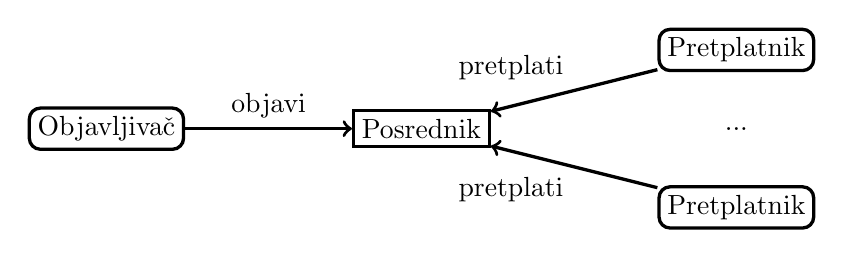
\begin{tikzpicture}[ % has a lot of options; consult the pgf manual
bend angle=45,
long_square/.style={rectangle, draw=black, fill=white, very thick, inner sep=3pt, minimum width=14mm},
rounded_square/.style={rectangle, rounded corners, draw=black, fill=white, very thick, inner sep=3pt, minimum width=14mm},
empty_circle/.style={rectangle, rounded corners=2mm, draw=black, fill=white, very thick, minimum size=4mm},
point/.style={circle, inner sep=0mm},
fit_square/.style={rectangle, rounded corners=2mm, draw=black, very thick, minimum height=32mm, minimum width=30mm},
both_arrow/.style={<->, very thick},
out_arrow/.style={->, very thick},
in_arrow/.style={<-, very thick},
above_edge_text/.style={above, midway, sloped}
]

\node[rounded_square](producer) at (0,0) {Objavljivač};

\node[long_square](broker) at (4,0) {Posrednik};

\node[rounded_square](consumer_1) at (8,1) {Pretplatnik};
\node[point](consumer_2) at (8,0) {...};
\node[rounded_square](consumer_3) at (8,-1) {Pretplatnik};



\draw[out_arrow](producer) to [] node[auto]{objavi} (broker);

\draw[out_arrow](consumer_1) to [] node[auto,swap]{pretplati} (broker);
\draw[out_arrow](consumer_3) to [] node[auto]{pretplati} (broker);

\end{tikzpicture}

\end{document}